%Įvade aprašomi darbo tikslai, nurodomas temos aktualumas, aptariamos teorinės
%darbo prielaidos bei metodologija, apibrėžiamas tiriamasis objektas,
%apibūdinami su tema susiję literatūros ar kitokie šaltiniai, temos analizės
%tvarka, darbo atlikimo aplinkybės, pateikiama žinių apie naudojamus
%instrumentus (programas ir kt.). Rekomenduojama įvado apimtis 3-4 puslapiai.

\sectionnonum{Įvadas}

% Kas yra biometrines identifikavimo sistemos
Kiekvieno žmogaus kūnas turi aibę požymių, pagal kuriuos jį galima unikaliai identifikuoti (pvz.: pirštų atspaudai).
Šių požymių egzistavimas davė pagrindą {\it biometrinėms identifikavimo sistemoms}.
Šių sistemų paskirtis yra tarp visų užregistruotų žmonių surasti tą, kuriam priklauso duotieji biometriniai požymiai.
Šiame darbe nagrinėjamoje sistemoje \cite{NeurotechnologyMegamatcherAccelerator} sąrašas žmonių, tarp kurių yra vykdoma paieška, yra papildomai atrenkamas pagal vartotojo pateiktą užklausą.
Ši užklausa sąrašą paieškai sudaro pagal papildomus, ne biometrinius, duomenis (pvz.: amžių, lytį, gyvenamąją vietą) priskirtus kiekvienam sistemoje užregistruotam žmogui.
Tokios užklausos vadinamos {\it biografinėmis užklausomis}.


% Kas yra biografinė užklausa ir biografiniai atributai?
\paragraph{Biografiniai atributai ir biografinė schema}

Aptartieji papildomi duomenys vadinami {\it biografiniais atributais}.
Verta atkreipti dėmesį į tai, kad šiame darbe biografiniai atributai yra supriešinami su biometriniais požymiais -- biografiniai atributai yra papildomi, būtinai ne biometriniai, duomenys.

Kiekvienas biografinis atributas turi savo vardą (pvz.: „Miestas“, „Amžius“), bei reikšmę (pvz.: „Vilnius“, „25-eri metai“).
Visų atributų vardų aibė yra vadinama {\it biografine schema}.
Pavyzdžiui \ref{tab:exampleGallery} lentelėje pateikiamame duomenų bazės pavyzdyje biografinė schema būtų \{„Miestas“, „Amžius“\}.

\begin{table}[H]\footnotesize
	\centering
	\begin{tabular}{|c|c|c|c|}
		\hline
		\multirow{2}{*}{{\bf Žmogus}} & \multirow{2}{*}{{\bf Biometriniai požymiai}} & \multicolumn{2}{|c|}{{\bf Biografiniai atributai}}  \\ \cline{3-4}
		& & {\bf Miestas} & {\bf Amžius} \\
		\hline
		Jonas  & biometrinių požymių įrašas & Vilnius & 25 \\ \cline{2-4}
		\hline
		Mindaugas & biometrinių požymių įrašas & Vilnius & 35 \\ \cline{2-4}
		\hline
		Petras & biometrinių požymių įrašas & Kaunas & 15 \\ \cline{2-4}
		\hline
		Eglė & biometrinių požymių įrašas & Klaipėda & 45 \\ \cline{2-4}
		\hline
	\end{tabular}
	\caption{Pavyzdiniai biometrinės identifikavimo sistemos duomenys}
	\label{tab:exampleGallery}
\end{table}

Kiekvienam žmogui gali būti priskiriamas daugiau negu vienas biografinis atributas, tačiau visiems žmonėms priskiriamų biografinių atributų schema turi būti tokia pati.
Tai reiškia, kad, pavyzdžiui, jeigu Jonui (žr.: \ref{tab:exampleGallery} lentelę) buvo priskirtas gyvenamasis miestas ir amžius, tai visiems likusiems užregistruotiems žmonės irgi bus priskiriamas gyvenamasis miestas ir amžius.

Nagrinėjama sistema palaiko dviejų tipų biografinius atributus:
\begin{itemize}
\item skaitinio tipo
\item simbolių eilutės tipo
\end{itemize}
Tačiau esant poreikiui šis sąrašas gali būti plečiamas.

Darbo metu bus daroma prielaida, kad tą patį vardą ir tipą turintiems atributams (pvz.: žmogaus amžiui) yra apibrėžta palyginimo funkcija (\ref{eq:threeWayComparisonFunction}).
\begin{equation}
	f(x_1, x_2)=
\begin{cases}
	-1,& \text{jeigu } x_1 < x_2\\
	0,& \text{jeigu } x_1 = x_2\\
	1,& \text{jeigu } x_1 > x_2\\
\end{cases}
\label{eq:threeWayComparisonFunction}
\end{equation}

Čia $x_1$ ir $x_2$ yra tą patį tipą ir vardą turinčio atributo reikšmės.

Taip pat darbe daroma prielaida, kad šios palyginimo funkcijos atžvilgiu atributo reikšmių aibė yra pilnai sutvarkyta \cite{hrbacek1999introduction}.






\paragraph{Duomenų bazės modelis}

Šiame darbe remiamasi duomenų bazės modeliu „Data cube“ \cite{marcel2000modeling}.
Nagrinėjamos sistemos atveju, daugiamatės erdvės ašys yra apibrėžiamos (\ref{eq:threeWayComparisonFunction}) funkcijos, taip kad:

\begin{equation}
	f(x_1, x_2)=-1
\label{eq:increasingOrderOfAtributes}
\end{equation}

visiems $x_1$, $x_2$ kur $x_1$ ašyje yra „mažesnėje“ (pvz.: kairiau atributo 1 ašyje \ref{img:multidimensionalGallery} pav.) pozicijoje $x_2$ atžvilgiu.

Žmonėms priskiriamų biografinių atributų reikšmių rinkiniai yra nagrinėjami kaip taškai šioje erdvėje.

\begin{figure}[H]
\begin{center}
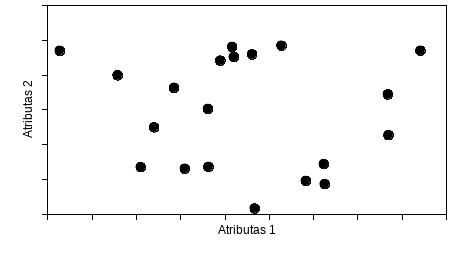
\includegraphics[width=0.5\textwidth]{img/MultidimensionalGallery.png}
\caption{Pavyzdiniai biografinių atributų rinkiniai dvimatėje erdvėje.}
\label{img:multidimensionalGallery}
\end{center}
\end{figure}

\ref{img:multidimensionalGallery} paveikslėlyje pateikiamas tokios erdvės pavyzdys.
Pavyzdyje palyginimo funkcija (\ref{eq:threeWayComparisonFunction}) atributo 1 (kuris yra skaitinio tipo) reikšmes palygina pagal sveikų skaičių tvarką.
O atributo 2 (kuris yra simbolių eilutės tipo) reikšmes palygina pagal leksikografinę tvarką.




% Biometrinių įrašų blokai - particijos daugiamatėje erdvėje
\paragraph{Biometrinių įrašų blokai daugiamatėje erdvėje}

Nagrinėjamoje sistemoje žmogaus biometrinių požymių įrašai saugomi ir apdorojami ne po vieną, bet grupėmis.
Šios grupės yra vadinamos {\it biometrinių įrašų blokais}.
Kiekvienam įrašui registracijos metu yra laisvai parenkamas vienas blokas, kuriame jis bus saugomas.

Šiame darbe nagrinėjamame duomenų bazės modelyje biometrinių įrašų blokai yra ankščiau aptartos daugiamatės erdvės sritys, kurios apima visus konkrečiam blokui priskirtus įrašus (žr.: \ref{img:multidimensionalPartitionedGallery} pav.)

\begin{figure}[H]
\begin{center}
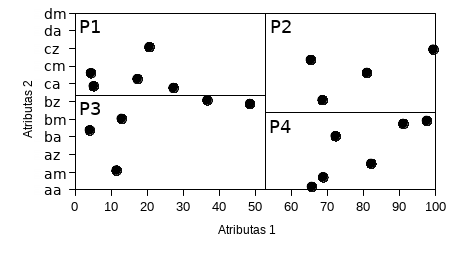
\includegraphics[width=0.5\textwidth]{img/MultidimensionalPartitionedGallery.png}
\caption{B1-B4 - erdvės sritys atitinkančios biometrinių įrašų blokus}
\label{img:multidimensionalPartitionedGallery}
\end{center}
\end{figure}



\paragraph{Biografinės užklausos}

Sistemoje žmonių sąrašas paieškai sudaromas pagal vartotojo užklausą.
Šiai užklausai aprašyti yra skirta gramatika, kurios Backus ir Nauro forma \cite{mccracken2003backus} yra pateikiama \ref{tab:queryBNF} lentelėje.

\begin{table}[H]\footnotesize
	\centering
	\begin{tabular}{|l c l|}
		\hline
		užklausa                      & ::= & <vienaris operatorius> <operandas> | \\
									  &     & \multicolumn{1}{l|}{<operandas> <dvinaris operatorius> <operandas> |} \\
									  &     & \multicolumn{1}{l|}{"(" <užklausa> ")" |} \\
									  &     & \multicolumn{1}{l|}{ <atributo vardas> <sąrašo operatorius> <sąrašas>} \\
		operandas                     & ::= & <užklausa> | <atributo vardas> | "'" <skaičius> "'" | "'" <žodis> "'" \\
		vienaris operatorius          & ::= & <neprivalomas tarpas> "NOT" <neprivalomas tarpas> \\
		dvinaris operatorius          & ::= & <neprivalomas tarpas> <dvinario operatoriaus ženklas> <neprivalomas tarpas> \\
		dvinario operatoriaus ženklas & ::= & ">" | ">=" | "<" | "<=" | "=" | "<>" | "AND" | "OR" \\
		sąrašo operatorius            & ::= & <neprivalomas tarpas> "IN" <neprivalomas tarpas> \\
		sąrašas                       & ::= & "(" <sąrašo elementai> ")" \\
		sąrašo elementai              & ::= & <sąrašo elementas> | <sąrašo elementas> "," <sąrašo elementai> \\
		sąrašo elementas              & ::= & "'" <žodis> "'" | "'" <skaičius> "'" \\
		atributo vardas               & ::= & <neprivalomas tarpas> <žodis> <neprivalomas tarpas> \\
		neprivalomas tarpas           & ::= & "" | " " <neprivalomas tarpas> \\
		žodis                         & ::= & <raidė> | <žodis> <raidė> | <žodis> <skaičius> \\
		skaičius                      & ::= & "0" | "1" | "2" | "3" | "4" | "5" | "6" | "7" | "8" | "9" \\
		raidė                         & ::= & "A" | "B" | "C" ... "Z" | "a" | "b" | "c" ... "z"  \\
		\hline
	\end{tabular}
	\caption{Biografinės užklausos aprašymo kalbos Backus ir Nauro forma}
	\label{tab:queryBNF}
\end{table}

Keletas užklausos pavyzdžių pateikiama \ref{tab:queryExamples} lentelėje laikant, kad biografinė schema yra \{„Miestas“, „Amžius“\}.

\begin{table}[H]\footnotesize
	\centering
	\begin{tabular}{|c|c|l|}
		\hline
		& {\bf Užklausos aprašymas} & {\bf Užklausos interpretacija} \\
		\hline
		Pavyzdys 1 & Amžius >= '18' & Visi suaugę žmonės\\
		\hline
		Pavyzdys 2 & Amžius >= '18' AND Miestas IN ('Vilnius', 'Kaunas') & Visi suagę vilniečiai ir kauniečiai\\
		\hline
		Pavyzdys 3 & NOT (Miestas = 'Vilnius' AND Amžius >= '18') & Visi žmonės išskyrus suaugusius vilniečius\\
		\hline
	\end{tabular}
	\caption{Užklausų aprašymo pavyzdžiai.}
	\label{tab:queryExamples}
\end{table}



\paragraph{Biografinių užklausų apdorojimas}

Smulkiausias žmonių sąrašas kuriame nagrinėjama sistema gali vykdyti paiešką yra vienas biometrinių įrašų blokas.
Todėl vartotojo užklausos apdorojimas yra skaidomas į tokius tris etapus:
\begin{enumerate}
	\item Atmetimo etapas: Atmetami visi blokai, kuriuose negali būti žmonių, kurių atributų rinkiniai atitinka vartotojo užklausą.
	\item Paieškos etapas: Atliekama paieška blokuose, kurie liko po atmetimo etapo.
	\item Filtravimo etapas: Atmetami visi paieškos etape rasti žmonės, kurių atributų rinkiniai neatitinka vartotojo užklausos.
\end{enumerate}

Verta pastebėti, kad po atmetimo etapo likęs blokų kiekis priklauso nuo metodo, pagal kurį yra parenkama daugiamatės erdvės sritis atributų rinkinių saugojimui.



\paragraph{Darbo tikslas}

Šio darbo metu siekiama padidinti biometrinės identifikavimo sistemos \cite{NeurotechnologyMegamatcherAccelerator} pralaidumą minimizuojant biometrinių įrašų blokų skaičių, kuris lieka po atmetimo etapo.

Šiuo tikslu bus įvertinami du metodai
\begin{itemize}
		\item Metodas paremtas priešdėliniu rūšavimu.
		\item Metodas paremtas K-d medžiu.
\end{itemize}

Darbą planuojama skirstyti į tokius uždavinius:

\begin{enumerate}
	\item Išanalizuoti tipinių užklausų statistines savybes, pasiruošti testavimo duomenis.
	\item Empiriškai įvertinti sistemos pralaidumo priklausomybę nuo įrašų skaičiaus bloke.
	\item Apibrėžti bei įvertinti metodą paremtą priešdėliniu rūšiavimu.
	\item Apibrėžti bei įvertinti metodą paremtą K-d medžiu.
\end{enumerate}

Šis darbas struktūrizuojamas taip:
I skyriuje apžvelgiami kiti panašūs darbai bei pateikiami šaltiniai, kuriais remiasi šis darbas.
II skyriuje nagrinėjamos užklausos.
Aptariama kokios užklausų savybės išplaukia iš apibrėžtos gramatikos, kokiomis statistinėmis savybėmis pasižymi vartotojų dažniausiai pateikiamos užklausos.
III skyriuje aprašoma kaip bus palyginami įrašų priskyrimo sritims metodai, bei aprašomas testavimo duomenų rinkinys.
IV skyriuje empiriškai nustatoma sistemos pralaiduomo priklausomybė nuo maksimalaus bloko dydžio.
Parenkamas bloko dydis, kuris bus naudojamas palyginant metodus.
V skyriuje apibrėžiamas metodas paremtas priešdėliniu rūšiavimu, įvertinamas jo efektyvumas.
VI skyriuje apibrėžiamas metodas paremtas K-d medžiu, įvertinamas jo efektyvumas.
Ir galiausiai aprašomi pasiekti rezultatai bei pateikiamos išvados.


